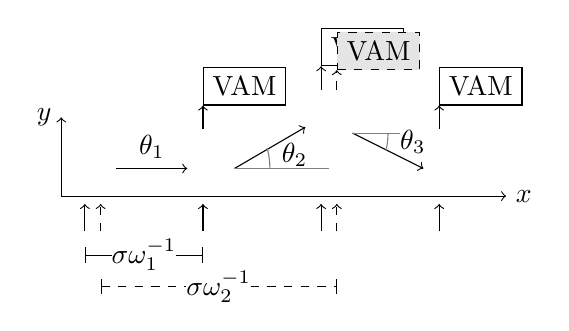
\begin{tikzpicture}
    % Distance delta
    \def\D{1.5}
    \def\xzero{.4}
    \def\yzero{.7}

    \draw[->] (0,0) -- (\xzero+3.5*\D,0)
        node[anchor=west] {$x$};
    \draw[->] (0,0) -- (0, 1)
        node[anchor=east] {$y$};

    % Pelaos' xcoordinates
    \def\xpone{\xzero}
    \def\xptwo{\xzero+\D}
    \def\xpthree{\xzero+2*\D}
    \def\xpfour{\xzero+3*\D}
    \def\cabeza{.15}

    % Stickmans/pelaos
    \pelao{\xpone}{\yzero}{\cabeza}
    \pelao{\xptwo}{\yzero}{\cabeza}
    \pelao{\xpthree}{\yzero+.5}{\cabeza}
    \pelao{\xpfour}{\yzero}{\cabeza}

    %%%%%%%%%%%%
    %% Angles %%
    %%%%%%%%%%%%
    % Angle1
    \draw[->] (\xpone+.3,.5*\yzero)
        -- (\xptwo-.3,.5*\yzero)
        node[midway,above] {$\theta_1$};
    % Angle2
    \draw[->] (\xptwo+.3,.5*\yzero)
        -- (\xpthree-.3,1.25*\yzero)
        node[pos=.85,below] {$\theta_2$};
    \draw[thin,gray] (\xptwo+.3,.5*\yzero)
        -- (\xpthree,.5*\yzero);
    \draw[gray] (\xptwo+.75,.5*\yzero)
        arc (0:15:1);
    % Angle3
    \draw[->] (\xpthree+.3,.1+\yzero)
        -- (\xpfour-.3,.5*\yzero)
        node[pos=.85,above] {$\theta_3$};
    \draw[thin,gray] (\xpthree+.3,.1+\yzero)
        -- (\xpthree+.9,.1+\yzero);
    \draw[gray] (\xpthree+.75,.1+\yzero)
        arc (0:-13:1);

    % GPS checks
    \def\arrlen{.35}
    \def\arrend{-.1}

    % High freq checks
    \draw[->] (\xpone-.1, \arrend-\arrlen)
        -- (\xpone-.1, \arrend);
    \draw[->] (\xptwo-.1, \arrend-\arrlen)
        -- (\xptwo-.1, \arrend);
    \draw[->] (\xpthree-.1, \arrend-\arrlen)
        -- (\xpthree-.1, \arrend);
    \draw[->] (\xpfour-.1, \arrend-\arrlen)
        -- (\xpfour-.1, \arrend);

    % Low freq checks
    \draw[->,dashed]
        (\xpone+.1, \arrend-\arrlen)
        -- (\xpone+.1, \arrend);
    \draw[->,dashed]
        (\xpthree+.1, \arrend-\arrlen)
        -- (\xpthree+.1, \arrend);

    % Intervals
    \draw[|-|] (\xpone-.1, \arrend-\arrlen-.3)
        --
        (\xptwo-.1, \arrend-\arrlen-.3)
        node[midway,fill=white,inner sep=0]
        {$\sigma\omega_1^{-1}$};
    \draw[|-|,dashed]
        (\xpone+.1, \arrend-\arrlen-.7)
        --
        (\xpthree+.1, \arrend-\arrlen-.7)
        node[midway,fill=white,inner sep=0]
        {$\sigma\omega_2^{-1}$};


    %%%%%%%%
    % VAMs
    %%%%%%%%
    % VAM1
    \node[draw,anchor=south west] (VAM1)
        at (\xptwo-.1, \yzero+\cabeza+.3)
        {VAM};
    \draw[->] (\xptwo-.1, \yzero+\cabeza)
        -- (VAM1.south west);
    % VAM2
    \node[draw,anchor=south west] (VAM2)
        at (\xpthree-.1, .5+\yzero+\cabeza+.3)
        {VAM};
    \draw[->] (\xpthree-.1, .5+\yzero+\cabeza)
        -- (VAM2.south west);
    % VAM2'
    \node[draw,anchor=south west,dashed,
        fill=gray!20!white] (VAM2p)
        at (\xpthree+.1, .5+\yzero+\cabeza+.25)
        {VAM};
    \draw[->,dashed]
        (\xpthree+.1, .5+\yzero+\cabeza)
        -- (VAM2p.south west);
    % VAM3
    \node[draw,anchor=south west] (VAM3)
        at (\xpfour-.1, \yzero+\cabeza+.3)
        {VAM};
    \draw[->] (\xpfour-.1, \yzero+\cabeza)
        -- (VAM3.south west);
\end{tikzpicture}


